\adjustmtc
\chapter[Systèmes linéaires, continus\ldots]{Systèmes linéaires continus et invariants\label{chap-SLCI}}     

\minitoc
\newpage


%%%%%%%%%%%%%%%%%%%%%%%%%%%%%%%%%%%%%%%%%%%%%%%%%%%%%%%%%%%%%%%%%%%%%ù
\section{Introduction}
%%%%%%%%%%%%%%%%%%%%%%%%%%%%%%%%%%%%%%%%%%%%%%%%%%%%%%%%%%%%%%%%%%%%%ù


%%%%%%%%%%%%%%%%%%%%%%%%%%%%%%%%%%%%%%%%%%%%%%%%%%%%%%%%%%%%%%%%%%%%%ù
\subsection{Système}
%%%%%%%%%%%%%%%%%%%%%%%%%%%%%%%%%%%%%%%%%%%%%%%%%%%%%%%%%%%%%%%%%%%%%ù
\begin{center}
    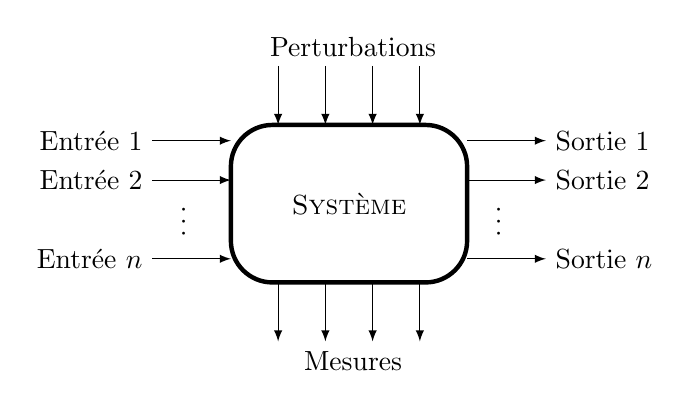
\begin{tikzpicture}
        \draw[-latex] (0.6,2.75) -- (0.6,2.0); 
        \draw[-latex] (1.2,2.75)node[above,xshift=1em] {Perturbations} -- (1.2,2.0); 
        \draw[-latex] (1.8,2.75) -- (1.8,2.0); 
        \draw[-latex] (2.4,2.75) -- (2.4,2.0); 
        \draw[ultra thick,rounded corners=15pt] (0,0) rectangle (3,2);
        \node (S) at (1.5,1) {\scshape Système};
        \draw[-latex] (-1,1.8) node[left] {Entrée 1} -- (0,1.8);
        \draw[-latex] (-1,1.3) node[left] {Entrée 2} -- (0,1.3);
        \node[] at (-0.6,0.8) {\rotatebox{90}{\ldots}};
        \draw[-latex] (-1,0.3) node[left] {Entrée $n$} -- (0,0.3);
        \draw[-latex] (3,1.8) -- (4,1.8)node[right] {Sortie 1};
        \draw[-latex] (3,1.3) -- (4,1.3)node[right] {Sortie 2};
        \node[] at (3.4,0.8) {\rotatebox{90}{\ldots}};
        \draw[-latex] (3,0.3) -- (4,0.3)node[right] {Sortie $n$};
        \draw[-latex] (0.6,0.0) -- (0.6,-0.75); 
        \draw[-latex] (1.2,0.0) -- (1.2,-0.75) node[below,xshift=1em] {Mesures}; 
        \draw[-latex] (1.8,0.0) -- (1.8,-0.75); 
        \draw[-latex] (2.4,0.0) -- (2.4,-0.75); 
    \end{tikzpicture}
\end{center}

%%%%%%%%%%%%%%%%%%%%%%%%%%%%%%%%%%%%%%%%%%%%%%%%%%%%%%%%%%%%%%%%%%%%%ù
\subsection{Système linéaire}
%%%%%%%%%%%%%%%%%%%%%%%%%%%%%%%%%%%%%%%%%%%%%%%%%%%%%%%%%%%%%%%%%%%%%ù

%%%%%%%%%%%%%%%%%%%%%%%%%%%%%%%%%%%%%%%%%%%%%%%%%%%%%%%%%%%%%%%%%%%%%ù
\subsection{Système à temps continu}
%%%%%%%%%%%%%%%%%%%%%%%%%%%%%%%%%%%%%%%%%%%%%%%%%%%%%%%%%%%%%%%%%%%%%ù

%%%%%%%%%%%%%%%%%%%%%%%%%%%%%%%%%%%%%%%%%%%%%%%%%%%%%%%%%%%%%%%%%%%%%ù
\subsection{Système invariant}
%%%%%%%%%%%%%%%%%%%%%%%%%%%%%%%%%%%%%%%%%%%%%%%%%%%%%%%%%%%%%%%%%%%%%ù

%%%%%%%%%%%%%%%%%%%%%%%%%%%%%%%%%%%%%%%%%%%%%%%%%%%%%%%%%%%%%%%%%%%%%ù
\section{Modélisation d'un signal}
%%%%%%%%%%%%%%%%%%%%%%%%%%%%%%%%%%%%%%%%%%%%%%%%%%%%%%%%%%%%%%%%%%%%%
Un signal 


%%%%%%%%%%%%%%%%%%%%%%%%%%%%%%%%%%%%%%%%%%%%%%%%%%%%%%%%%%%%%%%%%%%%%
\subsection{Types de signaux}
%%%%%%%%%%%%%%%%%%%%%%%%%%%%%%%%%%%%%%%%%%%%%%%%%%%%%%%%%%%%%%%%%%%%%ù
\acpl
Analogique, numérique et discret.
%%%%%%%%%%%%%%%%%%%%%%%%%%%%%%%%%%%%%%%%%%%%%%%%%%%%%%%%%%%%%%%%%%%%%
\subsection{Propriétés générales des signaux analogiques}
%%%%%%%%%%%%%%%%%%%%%%%%%%%%%%%%%%%%%%%%%%%%%%%%%%%%%%%%%%%%%%%%%%%%%ù

Un signal d'entrée ou de sortie d'un \SLCI~sera modélisé par 
une fonction continue du temps. Formellement, par une fonction $s$ telle que :

\begin{align*}
	s : \mathbb{R}&\rightarrow\mathbb{R} \\
	t&\rightarrow s(t) 
\end{align*}

\paragraph{Causal}

\begin{center}
    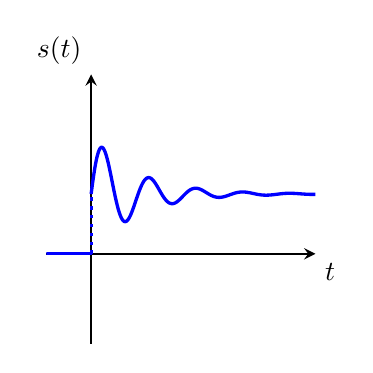
\begin{tikzpicture}
        \begin{axis}[
        axis line style = thick,
	ticks=none,
        height=5cm,
        width=5cm,
        axis x line=center,
        axis y line=center,
        xmin=-2,
        xmax=10,
        ymin=-1.5,
        ymax=3.0,
        xlabel={$t$},
        ylabel={$s(t)$},
        xlabel style={below right},
        ylabel style={above left},
        ]
        \addplot [very thick,color=blue,domain=-2:0, samples=101,unbounded coords=jump]{0};                                
	\addplot [very thick,color=blue,domain=0:10, samples=501,unbounded coords=jump]{sin(3*deg(x))*exp(-0.5*x)+1};
        \draw[dotted,very thick,blue] (axis cs:0,0) -- (axis cs:0,1); 
        \end{axis}
    \end{tikzpicture}
\end{center}


\paragraph{Stable}

\begin{center}
    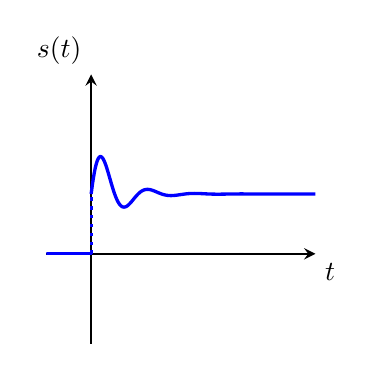
\begin{tikzpicture}
        \begin{axis}[
	ticks=none,
        axis line style = thick,
        height=5cm,
        width=5cm,
        axis x line=center,
        axis y line=center,
        xmin=-2,
        xmax=10,
        ymin=-1.5,
        ymax=3.0,
        xlabel={$t$},
        ylabel={$s(t)$},
        xlabel style={below right},
        ylabel style={above left},
        ]                                                                                                                     
        \addplot [very thick,color=blue,domain=-2:0, samples=101,unbounded coords=jump]{0};                                
	\addplot [very thick,color=blue,domain=0:10, samples=501,unbounded coords=jump]{sin(3*deg(x))*exp(-x)+1};                                
	\draw[dotted,very thick,blue] (axis cs:0,0) -- (axis cs:0,1); 
        \end{axis}                                                                                                            
    \end{tikzpicture}                                                                                                         
\end{center}                

\begin{center}
    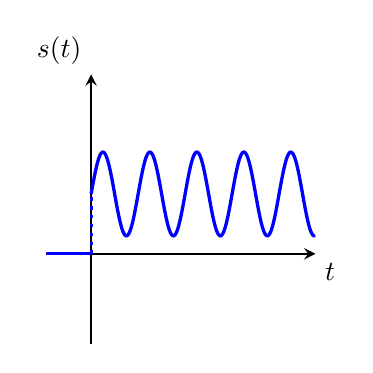
\begin{tikzpicture}
        \begin{axis}[
	ticks=none,
        axis line style = thick,
        height=5cm,
        width=5cm,
        axis x line=center,
        axis y line=center,
        xmin=-2,
        xmax=10,
        ymin=-1.5,
        ymax=3.0,
        xlabel={$t$},
        ylabel={$s(t)$},
        xlabel style={below right},
        ylabel style={above left},
        ]                                                                                                                     
        \addplot [very thick,color=blue,domain=-2:0, samples=101,unbounded coords=jump]{0};
	\addplot [very thick,color=blue,domain=0:10, samples=501,unbounded coords=jump]{0.7*sin(3*deg(x))+1};
	\draw[dotted,very thick,blue] (axis cs:0,0) -- (axis cs:0,1);
        \end{axis}
    \end{tikzpicture}
\end{center}

\begin{center}
    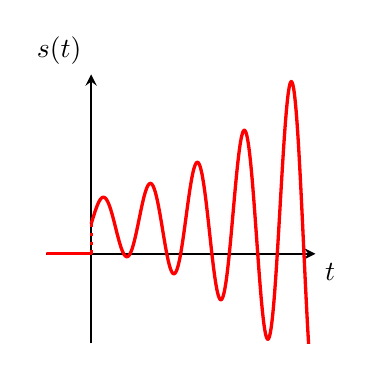
\begin{tikzpicture}
        \begin{axis}[
	ticks=none,
        axis line style = thick,
        height=5cm,
        width=5cm,
        axis x line=center,
        axis y line=center,
        xmin=-2,
        xmax=10,
        ymin=-3,
        ymax=6.0,
        xlabel={$t$},
        ylabel={$s(t)$},
        xlabel style={below right},
        ylabel style={above left},
        ]
        \addplot [very thick,color=red,domain=-2:0, samples=101,unbounded coords=jump]{0};
	\addplot [very thick,color=red,domain=0:10, samples=501,unbounded coords=jump]{0.8*sin(3*deg(x))*exp(0.2*x)+1};
	\draw[dotted,very thick,red] (axis cs:0,0) -- (axis cs:0,1);
        \end{axis}
    \end{tikzpicture}
\end{center}
\paragraph{Périodique}

\begin{center}
    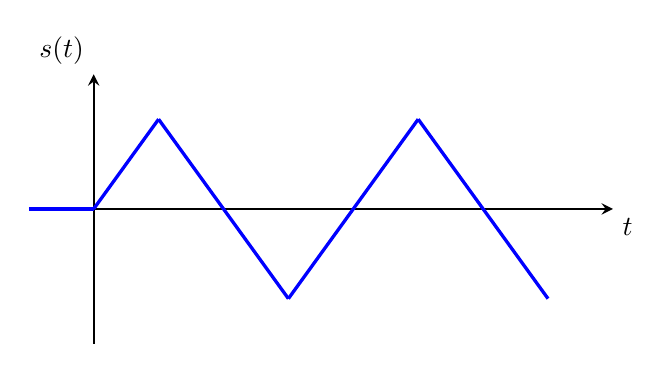
\begin{tikzpicture}
        \begin{axis}[
	ticks=none,
        axis line style = thick,
        height=5cm,
        width=9cm,
        axis x line=center,
        axis y line=center,
        xmin=-2,
        xmax=16,
        ymin=-1.5,
        ymax=1.5,
        xlabel={$t$},
        ylabel={$s(t)$},
        xlabel style={below right},
        ylabel style={above left},
        ]
        \addplot [very thick,color=blue,domain=-2:0, samples=101,unbounded coords=jump]{0};
        \addplot [very thick,color=blue,domain=0:2, samples=101,unbounded coords=jump]{0.5*x};
        \addplot [very thick,color=blue,domain=2:6, samples=101,unbounded coords=jump]{-0.5*x+2};
        \addplot [very thick,color=blue,domain=6:10, samples=101,unbounded coords=jump]{0.5*x-4};
        \addplot [very thick,color=blue,domain=10:14, samples=101,unbounded coords=jump]{-0.5*x+6};
        \end{axis}
    \end{tikzpicture}
\end{center}
%%%%%%%%%%%%%%%%%%%%%%%%%%%%%%%%%%%%%%%%%%%%%%%%%%%%%%%%%%%%%%%%%%%%%ù
\subsection{Signaux usuels}
%%%%%%%%%%%%%%%%%%%%%%%%%%%%%%%%%%%%%%%%%%%%%%%%%%%%%%%%%%%%%%%%%%%%%ù
%%%%%%%%%%%%%%%%%%%%%%%%%%%%%%%%%%%%%%%%%%%%%%%%%%%%%%%%%%%%%%%%%%%%%%%%%%
\paragraph{Impulsion de Dirac}
%%%%%%%%%%%%%%%%%%%%%%%%%%%%%%%%%%%%%%%%%%%%%%%%%%%%%%%%%%%%%%%%%%%%%%%%%%

L'impulsion de Dirac $\delta(t)$ est une \og fonction\fg 
\footnote{Les guillemets sont essentiels pour ne pas se fâcher avec nos collègues mathématiciens.} telle que
\begin{align*}
\delta(t) : 
\begin{dcases}
	\int\limits_{-\infty}^{+\infty}	 \delta(t)\,\,\dd{t}&=1   \\
	\int\limits_{-\infty}^{+\infty}  \delta(t)f(t)\,\,\dd{t}&=f(0)	
\end{dcases}
\end{align*}

Graphiquement une impulsion de Dirac $\delta(t)$ est 
représentée par une flèche en $t=0$. La figure ci-dessous présente 
une impulsion de Dirac ainsi qu'une 
impulsion retardée de $\tau$ noté $\delta(t-\tau)$.

\begin{figure}[!h]
\begin{center}
    \begin{tikzpicture}
        \begin{axis}[
        name=ax0,
        ticks=none,
        axis line style = thick,
        height=5cm,
        width=5cm,
        axis x line=center,
        axis y line=center,
        xmin=-4,
        xmax=4,
        ymin=-1.5,
        ymax=3.0,
        xlabel={$t$},
        ylabel={$\delta(t)$},
        xlabel style={below right},
        ylabel style={above left},
        ]
	\draw[ultra thick,blue,-latex] (axis cs:0,0) -- (axis cs:0,2.0);
        \end{axis}
        \begin{axis}[
        at={(ax0.south east)}, 
        xshift=4        em,                
        axis line style = thick,
        height=5cm,
        width=5cm,
        axis x line=center,
        axis y line=center,
        xmin=-4,
        xmax=4,
        ymin=-1.5,
        ymax=3.0,
        xlabel={$t$},
        ylabel={$\delta(t-\tau)$},
        xlabel style={below right},
        ylabel style={above left},
        xtick={2},
        xticklabels={$\tau$},
        ytick={10},
        yticklabels={},
        ]
	\draw[ultra thick,blue,-latex] (axis cs:2,0) -- (axis cs:2,2.0);
        \end{axis}

    \end{tikzpicture}
\end{center}
    \caption{\label{fig-dirac}}
\end{figure}

Impulsion réelle :

\begin{figure}[!h]
\begin{center}
    \begin{tikzpicture}
        \begin{axis}[
        ticks=none,
        axis line style = thick,
        height=5cm,
        width=5cm,
        axis x line=center,
        axis y line=center,
        xmin=-2,
        xmax=6,
        ymin=-1.5,
        ymax=3.0,
        xlabel={$t$},
        ylabel={$\delta(t)$},
        xlabel style={below right},
        ylabel style={above left},
        ]
        \addplot [thick,color=blue,domain=-2:0, samples=101,unbounded coords=jump]{0};
        \addplot [thick,color=blue,domain=0:2 , samples=101,unbounded coords=jump]{0.5};
        \addplot [thick,color=blue,domain=2:5 , samples=101,unbounded coords=jump]{0};
	\draw[dotted,thick,blue] (axis cs:0,0) -- (axis cs:0,0.5);
	\draw[dotted,thick,blue] (axis cs:2,0.5) -- (axis cs:2,0);
        \addplot [thick,color=green,domain=-2:0, samples=101,unbounded coords=jump]{0};
        \addplot [thick,color=green,domain=0:1 , samples=101,unbounded coords=jump]{1};
        \addplot [thick,color=green,domain=1:5 , samples=101,unbounded coords=jump]{0};
	\draw[dotted,thick,green] (axis cs:0,0) -- (axis cs:0,1);
	\draw[dotted,thick,green] (axis cs:1,1) -- (axis cs:1,0);
        \addplot [thick,color=red,domain=-2:0, samples=101,unbounded coords=jump]{0};
        \addplot [thick,color=red,domain=0:0.5 , samples=101,unbounded coords=jump]{2};
        \addplot [thick,color=red,domain=0.5:5 , samples=101,unbounded coords=jump]{0};
	\draw[dotted,thick,red] (axis cs:0,0) -- (axis cs:0,2);
	\draw[dotted,thick,red] (axis cs:0.5,2) -- (axis cs:0.5,0);
        \end{axis}
    \end{tikzpicture}
\end{center}
    \caption{\label{fig-dirac2}}
\end{figure}

La réponse à une impulsion de Dirac est appelée \textbf{réponse impulsionnelle}.

%%%%%%%%%%%%%%%%%%%%%%%%%%%%%%%%%%%%%%%%%%%%%%%%%%%%%%%%%%%%%%%%%%%%%%%%%%
\paragraph{\'Echelon unité}
%%%%%%%%%%%%%%%%%%%%%%%%%%%%%%%%%%%%%%%%%%%%%%%%%%%%%%%%%%%%%%%%%%%%%%%%%%

L'échelon unitaire est défini par la fonction, noté $u(t)$, telle que :
$$
u(t)=
\begin{cases} 
0 \qquad \forall t<0    \\ 
1 \qquad \forall t\geq 0 
\end{cases}
$$

Graphiquement, la fonction est représenté par une marche\footnote{Nos collègues 
anglo-saxons l'appelle la \og\emph{step function}\fg} à $t=0$. 
Ci dessous nous la représentons avec la fonction retardée $u(t-\tau)$.
\begin{figure}[!h]
\begin{center}
    \begin{tikzpicture}
        \begin{axis}[
        name=ax2,
        axis line style = thick,
        height=5cm,
        width=5cm,
        axis x line=center,
        axis y line=center,
        xmin=-2,
        xmax=6,
        ymin=-1.5,
        ymax=1.5,
        ytick={1},
        yticklabels={$1$},
        xtick=\empty,
        xlabel={$t$},
        ylabel={$u(t)$},
        xlabel style={below right},
        ylabel style={above left},
        ]
        \addplot [ultra thick,color=blue,domain=-2:0, samples=101,unbounded coords=jump]{0};
        \addplot [ultra thick,color=blue,domain=0:16, samples=101,unbounded coords=jump]{1};
	\draw[dotted,ultra thick,blue] (axis cs:0,0) -- (axis cs:0,1);
        \end{axis}
        \begin{axis}[
        at={(ax2.south east)},
        xshift=4em,
        ytick=\empty,
        axis line style = thick,
        height=5cm,
        width=5cm,
        axis x line=center,
        axis y line=center,
        xmin=-2,
        xmax=6,
        ymin=-1.5,
        ymax=1.5,
        ytick={1},
        yticklabels={$1$},
        xlabel={$t$},
        ylabel={$u(t-\tau)$},
        xlabel style={below right},
        ylabel style={above left},
	xticklabels={$\tau$},
        xtick={2},
        ]
        \addplot [ultra thick,color=blue,domain=-2:2, samples=101,unbounded coords=jump]{0};
        \addplot [ultra thick,color=blue,domain=2:16, samples=101,unbounded coords=jump]{1};
	\draw[dotted,ultra thick,blue] (axis cs:2,0) -- (axis cs:2,1);
        \end{axis}
    \end{tikzpicture}
\end{center}
\caption{\label{fig-echelon}}
\end{figure}

En général, l'échelon unitaire est utilisé en entrée de nos systèmes pour 
modéliser des états fermé/ouvert (\og on/off\fg).
Nous la rencontrerons souvent sous sa forme généralisée, 
$$
e(t)=E_0u(t)
$$
où $e(t)$ est le signal d'entrée du système et $E_0$ la valeur seuil de l'échelon dont 
l'unité dépend de la nature du problème considéré.

La réponse à un échelon est appelée \textbf{réponse indicielle}.


%%%%%%%%%%%%%%%%%%%%%%%%%%%%%%%%%%%%%%%%%%%%%%%%%%%%%%%%%%%%%%%%%%%%%%%%%%
\paragraph{Rampe unité}
%%%%%%%%%%%%%%%%%%%%%%%%%%%%%%%%%%%%%%%%%%%%%%%%%%%%%%%%%%%%%%%%%%%%%%%%%%

La fonction rampe\footnote{On retrouve parfois~\cite{sueurautomatique} le terme 
d'échelon vitesse pour désigner la fonction rampe} $r(t)$ unité est la fonction telle que :
$$
r(t)=
\begin{cases}
	0\,\,\,\,t<0 \\
	t\,\,\,\,t\geq0 
\end{cases}
$$
ou autrement dit, en utilisant la propriété de causalité de l'échelon:
$$
r(t)=t\cdot u(t)
$$

%%%%%%%%%%%%%%%%%%%%%%%%%%%%%%%%%%%%%%%%%%%%%%%%%%%%%%%%%%%%%%%%%%%%%%%%%%
\begin{figure}[!h]
%%%%%%%%%%%%%%%%%%%%%%%%%%%%%%%%%%%%%%%%%%%%%%%%%%%%%%%%%%%%%%%%%%%%%%%%%%
\begin{center}
    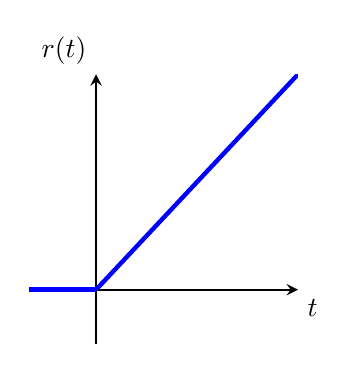
\begin{tikzpicture}
        \begin{axis}[
        ticks=none,
        axis line style = thick,
        height=5cm,
        width=5cm,
        axis x line=center,
        axis y line=center,
        xmin=-2,
        xmax=6,
        ymin=-1.5,
        ymax=6,
        xlabel={$t$},
        ylabel={$r(t)$},
        xlabel style={below right},
        ylabel style={above left},
        ]
        \addplot [ultra thick,color=blue,domain=-2:0, samples=101,unbounded coords=jump]{0};
        \addplot [ultra thick,color=blue,domain=0:15, samples=101,unbounded coords=jump]{x};
        \end{axis}
    \end{tikzpicture}
\end{center}
    \caption{\label{fig-rampe}}
\end{figure}
Remarquons que la fonction rampe est l'intégrale de l'échelon unité, notamment 
$$
r(t)=\int\limits_{-\infty}^{t} u(\tau)\,\,\dd{\tau}
$$

%%%%%%%%%%%%%%%%%%%%%%%%%%%%%%%%%%%%%%%%%%%%%%%%%%%%%%%%%%%%%%%%%%%%%%%%%%
\paragraph{Exponentielle décroissante}
%%%%%%%%%%%%%%%%%%%%%%%%%%%%%%%%%%%%%%%%%%%%%%%%%%%%%%%%%%%%%%%%%%%%%%%%%%
La fonction exponentielle décroissante $s(t)$ est telle que :
$$
s(t)=e^{-at}\cdot u(t)
$$  
avec $a$ l'inverse d'un temps caractéristique.

\begin{figure}[!h]
\begin{center}
    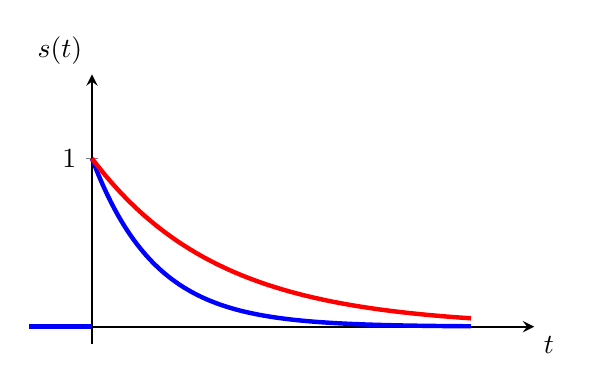
\begin{tikzpicture}
        \begin{axis}[
        axis line style = thick,
%        clip=false,
        height=5cm,
        width=8cm,
        axis x line=center,
        axis y line=center,
        xmin=-1,
        xmax=7,
        ymin=-0.1,
        ymax=1.5,
        xlabel={$t$},
        ylabel={$s(t)$},
        xlabel style={below right},
        ylabel style={above left},
        ytick={1},
        yticklabels={$1$},
        xtick=\empty,
        ]
            \addplot [ultra thick,color=blue,domain=-1:0, samples=101,unbounded coords=jump]{0};
            \addplot [ultra thick,color=blue,domain=0:6, samples=101,unbounded coords=jump]{exp(-x)};
            \addplot [ultra thick,color=red,domain=0:6, samples=101,unbounded coords=jump] {exp(-0.5*x)};
        \end{axis}
    \end{tikzpicture}
\end{center}
    \caption{\label{fig-exp}}
\end{figure}
%%%%%%%%%%%%%%%%%%%%%%%%%%%%%%%%%%%%%%%%%%%%%%%%%%%%%%%%%%%%%%%%%%%%%%%%%%
\paragraph{Sinuso\"ide}
%%%%%%%%%%%%%%%%%%%%%%%%%%%%%%%%%%%%%%%%%%%%%%%%%%%%%%%%%%%%%%%%%%%%%%%%%%
La fonction sinuso\"idale $s(t)$ est la fonction telle que :
$$
s(t)=A\sin{(\omega t +\phi)}\cdot u(t)
$$
avec $A$ son amplitude, $\omega$ sa pulsation (en rad/s) et $\phi$ sa phase (rad).
\begin{figure}[!h]
\begin{center}
    \begin{tikzpicture}
        \begin{axis}[
        axis line style = thick,
        clip=false,
        height=5cm,
        width=10cm,
        axis x line=center,
        axis y line=center,
        xmin=-2,
        xmax=4*pi,
        ymin=-1.5,
        ymax=1.5,
        xlabel={$t$},
        ylabel={$s(t)$},
        xlabel style={below right},
        ylabel style={above left},
        ytick={-1,1},
        yticklabels={$-A$,$A$},
        xtick={},
        xticklabels={},
        ]

            \addplot [ultra thick,color=blue,domain=-2:0, samples=101,unbounded coords=jump]{0};
            \addplot [ultra thick,color=blue,domain=0:4*pi, samples=101,unbounded coords=jump]{sin(deg(x))};
            \addplot [ultra thick,color=red,domain=0:4*pi, samples=101,unbounded coords=jump]{sin(deg(x-pi*0.5))};
            \draw[blue,] (axis cs:pi*0.5,1) -- (axis cs:pi*0.5,1.25);
            \draw[blue] (axis cs:pi*2.5,1) -- (axis cs:pi*2.5,1.25);
            \draw[blue,ultra thick, latex-latex] (axis cs:pi*0.5,1.2) --node[above,yshift=+0.2em]{$\dfrac{2\pi}{\omega}$} (axis cs:pi*2.5,1.2);
            \draw[blue,] (axis cs:pi*1.5,-1) -- (axis cs:pi*1.5,-1.25);
            \draw[blue] (axis cs:pi*1.5+pi*0.5,-1) -- (axis cs:pi*1.5+pi*0.5,-1.25);
            \draw[blue,ultra thick, latex-latex] (axis cs:pi*1.5,-1.2) --node[below,yshift=-0.2em]{$\dfrac{\Delta\phi}{\omega}$} (axis cs:pi*1.5+pi*0.5,-1.2);
        \end{axis}
    \end{tikzpicture}
\end{center}
\caption{\label{fig-sin}}
\end{figure}

La réponse à une sinuso\"ide est appelée la \textbf{réponse harmonique} 
et son analyse fera l'objet de tout un chapitre (\Cref{chap-anafreq}).

\newpage
%%%%%%%%%%%%%%%%%%%%%%%%%%%%%%%%%%%%%%%%%%%%%%%%%%%%%%%%%%%%%%%%%%%%%ù
\section{La transformée de Laplace}
%%%%%%%%%%%%%%%%%%%%%%%%%%%%%%%%%%%%%%%%%%%%%%%%%%%%%%%%%%%%%%%%%%%%%ù
La transformée de Laplace\footnote{Pierre-Simon de Laplace, (1749-1827) 
mathématicien, astronome, physicien et homme politique français} est l'outil indispensable 
pour l'étude des \SLCI. Celle-çi s'avère très utile pour 
la résolution d'équation différentielle régissant nos \SLCI~et nous permettra 
de définir la notion de fonction de transfert entre une entrée 
et une sortie d'un système.

%%%%%%%%%%%%%%%%%%%%%%%%%%%%%%%%%%%%%%%%%%%%%%%%%%%%%%%%%%%%%%%%%%%%%ù
\subsection{Définition}
%%%%%%%%%%%%%%%%%%%%%%%%%%%%%%%%%%%%%%%%%%%%%%%%%%%%%%%%%%%%%%%%%%%%%ù
La Transformée de Laplace (TL) d'une fonction causale $s$ (signal) 
d'une variable réelle $t$ (temps), est la fonction $S$ 
de la variable complexe $p$, définie par :
\begin{align}
S(p)=\laplace{s(t)}=\int_{0}^{+\infty} e^{-pt}s(t)\dd{t}.\label{eq-lap}
\end{align}


On dit également que \textbf{$S(p)$ est l'image dans le domaine de 
Laplace de la fonction $s(t)$ du domaine temporelle.}
De plus la transformée $S(p)$ de $s(t)$ est unique et parfaitement définie. 
Connaissant $S(p)$ on en déduit $s(t)$
par la transformation inverse 
$$
s(t)=\laplacei{S(p)}
$$
Les transformations inverse sont tabulées à l'\cref{annexe-lap}. Lorsque la transformation
n'existe pas dans les tables, on réalise une décompostion en éléments simple de la réponse 
$S(p)$ pour se placer dans un cas usuel (\cref{annexe-DES}).

Remarquons, dès à présent l'utilisation d'une convention utile: 
les fonctions du temps seront toujours désignées par une
minuscule, et les fonctions complexes par la majuscule respective.

%%%%%%%%%%%%%%%%%%%%%%%%%%%%%%%%%%%%%%%%%%%%%%%%%%%%%%%%%%%%%%%%%%%%%ù
\subsection{Transformées des signaux usuels}
%%%%%%%%%%%%%%%%%%%%%%%%%%%%%%%%%%%%%%%%%%%%%%%%%%%%%%%%%%%%%%%%%%%%%ù

%%%%%%%%%%%%%%%%%%%%%%%%%%%%%%%%%%%%%%%%%%%%%%%%%%%%%%%%%%%%%%%%%%%%%ù
\paragraph{Transformée d'une impulsion de Dirac}
%%%%%%%%%%%%%%%%%%%%%%%%%%%%%%%%%%%%%%%%%%%%%%%%%%%%%%%%%%%%%%%%%%%%%ù
Par simple application des définitions 
de la TL et de l'impulsion de Dirac, la transformée d'une 
impulsion de Dirac $\delta(t)$ s'écrit:
$$
\laplace{\delta(t)}=\int_{0}^{+\infty} e^{-pt}\,\delta(t)\dd{t}=1
$$
ou encore
\begin{bequation}[ams align]
    \laplace{\delta(t)}=1
\end{bequation}

%%%%%%%%%%%%%%%%%%%%%%%%%%%%%%%%%%%%%%%%%%%%%%%%%%%%%%%%%%%%%%%%%%%%%ù
\paragraph{Transformée d'un échelon unitaire}
%%%%%%%%%%%%%%%%%%%%%%%%%%%%%%%%%%%%%%%%%%%%%%%%%%%%%%%%%%%%%%%%%%%%%ù
La transformée de Laplace d'un signal échelon unitaire s'écrit : 
$$
\laplace{u(t)}=\int_{0}^{+\infty} e^{-pt}\,u(t)\dd{t}=\int_{0}^{+\infty} e^{-pt}\dd{t}=\left[\dfrac{-e^{-pt}}{p}\right]_0^{+\infty}=\dfrac{1}{p}
$$
ou encore
\begin{bequation}[ams align]
    \laplace{u(t)}=\dfrac{1}{p}
\end{bequation}
%Dans le cas de la forme généralisée, il suffit de multiplier par une constante.
%%%%%%%%%%%%%%%%%%%%%%%%%%%%%%%%%%%%%%%%%%%%%%%%%%%%%%%%%%%%%%%%%%%%%ù
\paragraph{Transformée d'une rampe}
%%%%%%%%%%%%%%%%%%%%%%%%%%%%%%%%%%%%%%%%%%%%%%%%%%%%%%%%%%%%%%%%%%%%%ù
La transformée de Laplace d'un signal rampe s'écrit :
$$
\laplace{r(t)}=\int_{0}^{+\infty} e^{-pt}r(t)\dd{t}=\int_{0}^{+\infty} te^{-pt}\dd{t}
$$
Par intégration par parties:
\begin{align*}
    v=-\dfrac{1}{p}e^{-pt}\qquad&\dd{u}=\dd{t}\\
    \dd{v}=e^{-pt}\dd{t}\qquad&u=t
\end{align*}
$$
\int_{0}^{+\infty} te^{-pt}\dd{t} = \left[-t\dfrac{1}{p}e^{-pt}\right]_0^{+\infty}-\int_{0}^{+\infty} -\dfrac{1}{p}e^{-pt}\dd{t}=\dfrac{1}{p^2}
$$
ou encore
\begin{bequation}[ams align]
    \laplace{r(t)}=\laplace{t\cdot u(t)}=\dfrac{1}{p^2}
\end{bequation}

%%%%%%%%%%%%%%%%%%%%%%%%%%%%%%%%%%%%%%%%%%%%%%%%%%%%%%%%%%%%%%%%%%%%%ù
\paragraph{Transformée d'une exponentielle décroissante}
%%%%%%%%%%%%%%%%%%%%%%%%%%%%%%%%%%%%%%%%%%%%%%%%%%%%%%%%%%%%%%%%%%%%%ù

$$
\laplace{e^{-at}u(t)}=\int_{0}^{+\infty} e^{-pt}e^{-at}\dd{t}=\int_{0}^{+\infty} e^{-(p+a)t}\dd{t} = \dfrac{1}{p+a}
$$
ou encore
\begin{bequation}[ams align]
    \laplace{e^{-at}u(t)}=\dfrac{1}{p+a}
\end{bequation}

%%%%%%%%%%%%%%%%%%%%%%%%%%%%%%%%%%%%%%%%%%%%%%%%%%%%%%%%%%%%%%%%%%%%%ù
\paragraph{Transformée d'une sinuso\"ide}
%%%%%%%%%%%%%%%%%%%%%%%%%%%%%%%%%%%%%%%%%%%%%%%%%%%%%%%%%%%%%%%%%%%%%ù
La transformée de Laplace d'un signal sinuso\"idal s'écrit :
\begin{align*}
    \laplace{\sin{\omega t}\cdot u(t)}&=\int_{0}^{+\infty}e^{-pt}\dfrac{e^{\jw t}-e^{-\jw t}}{2j}\dd{t}=\dfrac{1}{2j}\int_{0}^{+\infty}e^{-(p-\jw)t}\dd{t} - \int_{0}^{+\infty}e^{-(p+\jw)t}\dd{t} \\
 &=\dfrac{1}{2j}\left( \dfrac{1}{p-\jw}-\dfrac{1}{p+\jw}\right)\\
 &=\dfrac{\omega}{p^2+\omega^2}
\end{align*}
ou encore
\begin{bequation}[ams align]
    \laplace{\sin{\omega t}\cdot u(t)}=\dfrac{\omega}{p^2+\omega^2}
\end{bequation}



%%%%%%%%%%%%%%%%%%%%%%%%%%%%%%%%%%%%%%%%%%%%%%%%%%%%%%%%%%%%%%%%%%%%%ù
\subsection{Propriétés}
%%%%%%%%%%%%%%%%%%%%%%%%%%%%%%%%%%%%%%%%%%%%%%%%%%%%%%%%%%%%%%%%%%%%%ù
Nous allons ici uniquement présenter les principales propriétés de la TL, 
on se rapportera à nouveau à l'\cref{annexe-lap} pour 
une liste exhaustive de ces propriétés.

La propriété fondamentale de la transformée de Laplace est d'être linéaire.

%%%%%%%%%%%%%%%%%%%%%%%%%%%%%%%%%%%%%%%%%%%%%%%%%%%%%%%%%%%%%%%%%%%%%ù
\paragraph{Retard}
%%%%%%%%%%%%%%%%%%%%%%%%%%%%%%%%%%%%%%%%%%%%%%%%%%%%%%%%%%%%%%%%%%%%%ù
Soit $s(t-\tau)$ un signal $s(t)$ présentant un retard $\tau$.
$$
\laplace{s(t-\tau)}=\int_{0}^{+\infty} e^{-pt}s(t-\tau)\dd{t}
$$
en appliquant le changement de variable $t'=t-\tau$, on obtient $t=t'+\tau$ et $\dd{t}=\dd{t}$
$$
\laplace{s(t-\tau)}=\int_{\tau}^{+\infty} e^{-p(t'+\tau)}s(t')\dd{t'}=e^{-p\tau}\int_{0}^{+\infty} e^{-pt'}s(t')\dd{t'}=
$$
on reconnait dans cette dernière expression la définition de la transformée de Laplace, on écrit alors :
\begin{bequation}[ams align]
    \laplace{s(t-\tau)}=e^{-p\tau}S(p)
\end{bequation}
%%%%%%%%%%%%%%%%%%%%%%%%%%%%%%%%%%%%%%%%%%%%%%%%%%%%%%%%%%%%%%%%%%%%%
\paragraph{Dérivation}
%%%%%%%%%%%%%%%%%%%%%%%%%%%%%%%%%%%%%%%%%%%%%%%%%%%%%%%%%%%%%%%%%%%%%
Soit un signal $s(t)$ continu et dérivable pour $t\ge0$ et $S(p)$ sa transformée.
Par définition de la transformée de Laplace 
$$
\laplace{\devi{s(t)}{}}=\int_{0}^{+\infty} e^{-pt}\devi{s(t)}{}\dd{t}
$$
par intégration par parties
\begin{align*}
    v=e^{-pt}\qquad&\dd{u}=\devi{s(t)}{}\dd{t}\\
    \dd{v}=-pe^{-pt}\dd{t}\qquad&u=s(t)
\end{align*}
\begin{align*}
    \laplace{\devi{s(t)}{}}&=\left[s(t)e^{-pt}\right]_0^{+\infty}-p\int_{0}^{+\infty} e^{-pt}s(t)\dd{t} \\
                           &=f(0)+pS(p)
\end{align*}
ou encore
\begin{bequation}[ams align]
    \laplace{\devi{s(t)}{}}=pS(p)+f(0)
\end{bequation}
On généralise à tous les ordres de dérivation dans le cas de conditions initiales nulles.
$$
\laplace{\devi{s(t)}{n}}=p^nS(p)
$$

Remarquons que \textbf{dériver dans le domaine temporelle consiste à multiplier par 
$p$ dans le domaine de Laplace.}
%%%%%%%%%%%%%%%%%%%%%%%%%%%%%%%%%%%%%%%%%%%%%%%%%%%%%%%%%%%%%%%%%%%%%ù
\paragraph{Intégration}
%%%%%%%%%%%%%%%%%%%%%%%%%%%%%%%%%%%%%%%%%%%%%%%%%%%%%%%%%%%%%%%%%%%%%ù
Soient  des signaux $v(t)$ et $s(t)$ tel que $v(t)=\int_{0}^{t}s(\tau)\dd{\tau}$. 
Par définition,
$$
\laplace{v(t)}=\int_{0}^{+\infty} e^{-pt}v(t)\dd{t}
$$
par intégration par parties,
\begin{align*}
    v=v(t)\qquad&\dd{u}=e^{-pt}\dd{t}\\
    \dd{v}=s(t)\dd{t}\qquad&u=-\dfrac{1}{p}e^{-pt}
\end{align*} 
\begin{align*}
    \laplace{v(t)}&=\left[-\dfrac{1}{p}v(t)\right]_0^{+\infty}-\int_{0}^{+\infty} -\dfrac{1}{p}e^{-pt}s(t)\dd{t} \\
    &=\dfrac{1}{p}\int_{0}^{+\infty} e^{-pt}s(t)\dd{t}       
\end{align*}
ou encore
\begin{bequation}[ams align]
    \laplace{\int_{0}^{t}s(\tau)\dd{\tau}}=\dfrac{S(p)}{p}
\end{bequation}
Remarquons que \textbf{intégrer dans le domaine temporelle consiste à diviser par $p$ 
dans le domaine de Laplace.}


%%%%%%%%%%%%%%%%%%%%%%%%%%%%%%%%%%%%%%%%%%%%%%%%%%%%%%%%%%%%%%%%%%%%%ù
\paragraph{Théorème de la valeur initiale}
%%%%%%%%%%%%%%%%%%%%%%%%%%%%%%%%%%%%%%%%%%%%%%%%%%%%%%%%%%%%%%%%%%%%%ù
\begin{bequation}[ams align]
    s(0)=\lim\limits_{p\rightarrow+\infty} p S(p)\qquad \forall S(p)
\end{bequation}

%%%%%%%%%%%%%%%%%%%%%%%%%%%%%%%%%%%%%%%%%%%%%%%%%%%%%%%%%%%%%%%%%%%%%ù
\paragraph{Théorème de la valeur finale}
%%%%%%%%%%%%%%%%%%%%%%%%%%%%%%%%%%%%%%%%%%%%%%%%%%%%%%%%%%%%%%%%%%%%%ù
\begin{bequation}[ams align]
    s(\infty)=\lim\limits_{p\rightarrow0} p S(p)
\end{bequation}
valable que si $pS(p)$ a tous ses pôles à partie réelle strictement négative, autrement dit que le
signal soit stable.


%%%%%%%%%%%%%%%%%%%%%%%%%%%%%%%%%%%%%%%%%%%%%%%%%%%%%%%%%%%%%%%%%%%%%ù
\subsection[Application de la transformée de Laplace]{Application de la TL à la résolution d'équation différentielle}
%%%%%%%%%%%%%%%%%%%%%%%%%%%%%%%%%%%%%%%%%%%%%%%%%%%%%%%%%%%%%%%%%%%%%ù

Soit l'équation différentielle suivante :
\begin{align}
\devi{s(t)}{2}+2\devi{s(t)}{} + s(t) = e(t)\label{eq-diff1}
\end{align}

où $e(t)$ et $s(t)$ sont respectivement les fonctions temporelles d'entrée et de sortie du système
régit par cette équation différentielle avec pour conditions initiales (CI) 
$s(0)=-1$ et $s'(0)=2$.
Nous considérons la réponse à un échelon unitaire ( i.e $e(t)=u(t)$ ) 

Nous allons résoudre cette équation par deux méthodes différentes: la méthode classique 
de résolution d'équations différentielles avec second membre, 
et par l'application de la transformée de Laplace\footnote{Dans le cas particulier
de cette équation différentielle, on observera que la méthode classique est plus 
facile à mettre en oeuvre. Ceci n'est pas toujours le cas. 
Comme nous le verrons la transformée de Laplace devient totalement indispensable pour la 
définition de la fonction de transfert d'un \SLCI.}.
%%%%%%%%%%%%%%%%%%%%%%%%%%%%%%%%%%%%%%%%%%%%%%%%%%%%%%%%%%%%%%%%%%%%
\paragraph{Résolution par la méthode \og classique\fg}
%%%%%%%%%%%%%%%%%%%%%%%%%%%%%%%%%%%%%%%%%%%%%%%%%%%%%%%%%%%%%%%%%%%%
L'équation caractéristique associée à cette équation différentielle est donnée par 
$$
r^2+2r+1=0
$$
cette équation possède une solution double $r_{1,2}=-1$.
La solution homogène $s_0(t)$ est donc de la forme
$$
s_0(t)=(\alpha t+\beta)e^{-t}.
$$
Une solution particulière $s_1(t)=1$ nous est trivialement donnée par l'entrée en échelon qui correspond au 
régime permanent.
La solution générale est donc donnée par :
$$
s(t)=(\alpha t+\beta)e^{-t}+1
$$
Dérivons cette solution générale pour pouvoir déterminer les coéfficients $\alpha$, $\beta$ en utilisant
les conditions initiales,
$$
s'(t)=\alpha e^{-t}-(\alpha t+\beta)e^{-t}
$$

\begin{align*}
     s(0)&=-1\Rightarrow\beta+1=-1\Rightarrow\beta=-2 \\
    s'(0)&=\hphantom{-}2\Rightarrow\alpha+2=\hphantom{-}2\Rightarrow\alpha=0
\end{align*}

\begin{figure}[!t]
    \centering
    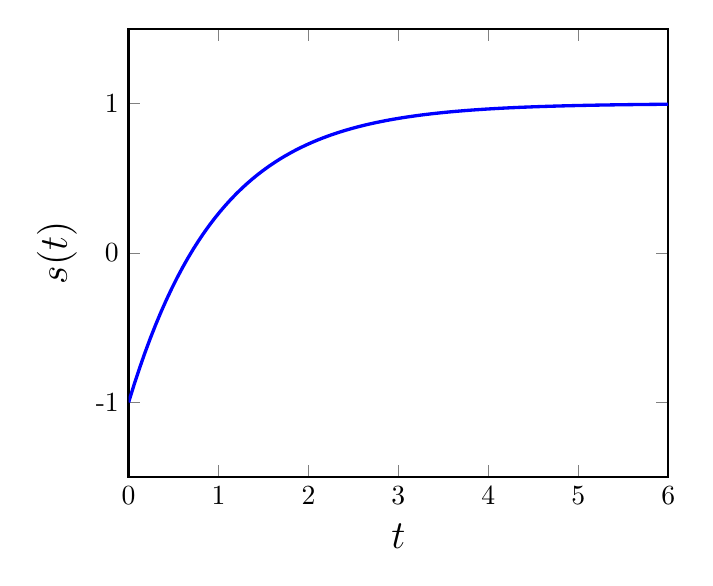
\begin{tikzpicture}%[baseline=0]
        \begin{axis}[
        scaled y ticks = false,
        axis line style = thick,
        %height=5cm,
        %width=9cm,
        %axis x line=center,
        %axis y line=center,
        xmin=0,
        xmax=6.0,
        ymin=-1.5,
        ymax=1.5,
        xlabel={$t$},
        ylabel={$s(t)$},
        %xlabel style={below right},
        %ylabel style={above left},
        yticklabels={-1,0,1},
        ytick={-1,0,1.0},
        y tick label style={anchor=east},
        label style={font=\Large},
        ]
        \addplot [very thick,color=blue,domain=0:6, samples=101,unbounded coords=jump]{1-2*exp(-x)};
        \end{axis}
    \end{tikzpicture}
    \caption{Représentation de la solution générale de l'équation différentielle~(\ref{eq-diff1}). On vérifie lors 
    du tracer que l'on observe bien les principales propriétes du signal (i.e conditions initiales, valeurs finales).}
\end{figure}

La solution générale de l'équation différentielle~(\ref{eq-diff1}) est donc 
\begin{bequation}[ams align]
s(t)=1-2e^{-t}
\end{bequation}
On constate que cette solution vérifie l'équation différentielle (\ref{eq-diff1}) ainsi que les 
conditions initiales.

%%%%%%%%%%%%%%%%%%%%%%%%%%%%%%%%%%%%%%%%%%%%%%%%%%%%%%%%%%%%%%%%%
\paragraph{Résolution par appliqation de la transformée de Laplace}
%%%%%%%%%%%%%%%%%%%%%%%%%%%%%%%%%%%%%%%%%%%%%%%%%%%%%%%%%%%%%%%%%

Appliquons la transformée de Laplace aux différents termes de l'équation différentielle~(\ref{eq-diff1}),
nous obtenons
\begin{align*}
    \laplace{s(t)} &= S(p) \\
    \laplace{\devi{s(t)}{}} &= pS(p)-s(0) = pS(p) +1 \\
    \laplace{\devi{s(t)}{2}} &= p^2S(p)-ps(0)-s'(0) = p^2S(p) + p -2\\
    \laplace{u(t)} &= \dfrac{1}{p}
\end{align*}

L'équation différentielle~(\ref{eq-diff1}) devient dans le domaine de Laplace :
\begin{align*}
p^2S(p)+p-2+2pS(p)+2+S(p)=\dfrac{1}{p} 
\end{align*}

En réarrangeant cette expression, il est possible de déterminer la forme de la réponse 
$S(p)$ dans le domaine de Laplace.

\begin{align*}
    S(p)\left(p^2+2p+1\right)+p&=\dfrac{1}{p} \\
    S(p)\left(p+1\right)^2 &= \dfrac{1-p^2}{p}\\
    S(p)&= \dfrac{1-p^2}{p\left(p+1\right)^2}
\end{align*}

Cette forme \og n'existant\fg pas dans les tableaux de transformation de Laplace usuels, nous allons décomposer cette
fraction rationnelle en éléments simples (\Cref{annexe-DES}).

$$
S(p)=\dfrac{A}{p}+\dfrac{B}{p+1}+\dfrac{C}{(p+1)^2}
$$

Par identification, 
$$
S(p)=\dfrac{A(p+1)^2+Bp(p+1)+Cp}{p(p+1)^2}=\dfrac{1-p^2}{p\left(p+1\right)^2}
$$

$$
\begin{cases}
    A+B&=-1 \\
    2A+B+C&=0 \\
    A&=1   
\end{cases}\Rightarrow
\begin{cases}
    B&=-2\\
    C&=0
\end{cases}
$$

La réponse $S(p)$ se décompose donc de la façon suivante en éléments simples:
$$
S(p)=\dfrac{1}{p}-\dfrac{2}{p+1}
$$
Il est maitenant plus aisé d'appliquer la transformation de Laplace inverse, 
en utilisant le tableau des transformées de Laplace usuels (\Cref{annexe-lap}) 
pour obtenir la réponse temporelle $s(t)$. Notamment,
$$
\laplacei{\dfrac{1}{p}}=1
$$
et
$$
\laplacei{\dfrac{2}{p+1}}=2e^{-t}
$$
soit 
\begin{bequation}[ams align]
    \laplacei{S(p)}=s(t)=1-2e^{-t}
\end{bequation}

Comme attendu, les deux méthodes donnent le même résultat, cependant la transformée de Laplace permet de définir dans 
le domaine de Laplace, une relation direct entre l'entrée et la sortie d'un système. C'est la fonction de transfert 
qui réalise ce lien.

%%%%%%%%%%%%%%%%%%%%%%%%%%%%%%%%%%%%%%%%%%%%%%%%%%%%%%%%%%%%%%%%%%%%%%%%%%%%%
\section{Fonction de Transfert}
%%%%%%%%%%%%%%%%%%%%%%%%%%%%%%%%%%%%%%%%%%%%%%%%%%%%%%%%%%%%%%%%%%%%%%%%%%%%%

Comme nous l'avons déjà discuté, un \SLCI~est par définition représenté par 
une équation différentielle 
à coefficients constants,

\begin{align}
    \sum_{i=0}^{n}a_i\devi{s(t)}{i}=\sum_{i=0}^{m}b_i\devi{e(t)}{i}\label{eq-ltemp}
\end{align}
avec $n,m\in\mathbb{N}$, $s(t)$ le signal de sortie, $e(t)$ le signal d'entrée et $a_i,b_i\in\mathbb{R}$.
L'équation est dite d'ordre $n$.

Sous cette forme, cette équation différentielle constitue ce que l'on nomme \textbf{la loi temporelle} du système.
Sans perte de généralité, on ne considèrera dans un premier temps 
que les systèmes pour lesquels toutes les 
\textbf{conditions initialles sont nulles}\footnote{Que l'on nomme la condition d'Heaviside}.

En appliquant la transformée de Laplace à l'\cref{eq-ltemp}, on obtient
\begin{align}
    \sum_{i=0}^{n}a_ip^iS(p)=\sum_{i=0}^{m}b_ip^iE(p)\label{eq-lfreq}
\end{align}
Sous cette forme, cette équation constitue ce que l'on nomme \textbf{la loi fréquentielle} du système.

%%%%%%%%%%%%%%%%%%%%%%%%%%%%%%%%%%%%%%%%%%%%%%%ù
\paragraph{Définition}
%%%%%%%%%%%%%%%%%%%%%%%%%%%%%%%%%%%%%%%%%%%%%%%ù

La fonction de transfert $H(p)$ d'un système est donnée par le rapport de la 
sortie $S(p)$ sur l'entrée $E(p)$. 
\begin{bequation}[ams align]
H(p)=\dfrac{S(p)}{E(p)}
\end{bequation}
Cette fonction $H(p)$ est également appelé transmittance.

%%%%%%%%%%%%%%%%%%%%%%%%%%%%%%%%%%%%%%%%%%%%%%%%%%%%%%%%%%%%%%%%%%%%%%%%%%%%%
\subsection[Représentation de la fonction de transfert]{Représentations algébrique et graphique de la fonction de transfert}
%%%%%%%%%%%%%%%%%%%%%%%%%%%%%%%%%%%%%%%%%%%%%%%%%%%%%%%%%%%%%%%%%%%%%%%%%%%%%

D'après la loi fréquentielle (\Cref{eq-lfreq}), la fonction de transfert 
d'un \SLCI~peut s'écrire sous la forme d'une fraction rationnelle,
\begin{bequation}[ams align]
H(p)=\dfrac{\sum\limits_{i=0}^{m}b_ip^i}{\sum\limits_{i=0}^{n}a_ip^i}. \label{eq-ftgen}
\end{bequation}

Il existe différentes façons équivalentes d'écrire cette fonction de transfert. 
Nous allons en introduire deux :
la forme canonique et la forme factorisée. La forme canonique permet de faire apparaître 
les intégrateurs purs du systèmes. La forme factorisée utilise les racines de la 
fraction rationnelle définissant la fonction de transfert. 
%Pour montrer l'équivalence de ces représentations nous allons les 
%construire à partir de la forme générale de l'\cref{eq-ftgen} et ou de la connaissance des pôles et zéros de 
%la fonction de transfert.

Une fonction de transfert peut être vue comme le fraction de deux polynômes (i.e fraction rationnelle):
un polynôme au numérateur $N(p)$ et un polynôme au dénominateur $D(p)$.
$$
H(p)=\dfrac{N(p)}{D(p)}
$$
Ces polynômes possèdent des racines dans $\mathbb{C}$. Les \textbf{racines de $N(p)$ sont 
dits les zéros de $H(p)$ }et les \textbf{racines de $D(p)$ 
sont dits les pôles de $H(p)$}. Il en vient qu'une fonction de transfert possède $m$ zéros et $n$ pôles.

%%%%%%%%%%%%%%%%%%%%%%%%%%%%%%%%%%%%%%%%%%%%%%%ù
\paragraph{Exemple}
%%%%%%%%%%%%%%%%%%%%%%%%%%%%%%%%%%%%%%%%%%%%%%%ù
Reprenons l'équation différentielle de la section précédente, dans les conditions de Heaviside, afin de construire 
la fonction de transfert qui lui est associée. 
\begin{align}                                                                                                                 
\devi{s(t)}{2}+2\devi{s(t)}{} + s(t) = e(t)  
\end{align}  
La transformée de Laplace de cette équation nous donne,
\begin{align*}                                        
	p^2S(p)+2pS(p)+S(p)&=E(p)\\
	S(p)\left(p^2+2p+1\right)&=E(p)\\
	S(p)&=\dfrac{1}{p^2+2p+1}E(p)
\end{align*}  
La fonction de transfert associée à cette équation différentielle est donc 
$$
H(p)=\dfrac{1}{p^2+2p+1}
$$
%Il est aisé de constater que la fonction de transfert est d'ordre deux et ne possède pas de zéro.


%%%%%%%%%%%%%%%%%%%%%%%%%%%%%%%%%%%%%%%%%%%%%%%ù
\paragraph{Forme canonique de la fonction de transfert}
%%%%%%%%%%%%%%%%%%%%%%%%%%%%%%%%%%%%%%%%%%%%%%%ù
Développons les sommes de l'\cref{eq-ftgen},
$$
H(p)=\dfrac{b_0+b_1p+b_2p^2+\ldots+b_mp^m}{a_0+a_1p+a_2p^2+\ldots+a_np^n}.
$$
La forme canonique dépend du nombre d'intégrateur du système. 
Par exemple, si $a_0$ est non nul, l'expression précédente se factorise sous la forme,
$$
H(p)=K_0\cdot\dfrac{1+b'_1p+b'_2p^2+\ldots+b'_mp^m}{1+a'_1p+a'_2p^2+\ldots+a'_np^n}.
$$
avec $K_0=\dfrac{b_0}{a_0}$, $a'_i=\dfrac{a_i}{a_0}$ et $b'_i=\dfrac{b_i}{b_0}$. 
Dans ce cas, le système est dit de classe 0 et donc ne possède aucun intégrateur.

Si maintenant $a_0$ est nul et $a_1$ non nul, la fonction de transfert peut s'écrire,
$$
H(p)=\dfrac{K_1}{p}\cdot\dfrac{1+b'_1p+b'_2p^2+\ldots+b'_mp^m}{1+a'_1p+a'_2p^2+\ldots+a'_{n-1}p^{n-1}}.
$$
avec $K_1=\dfrac{b_0}{a_1}$, $a'_i=\dfrac{a_{i+1}}{a_1}$ et $b'_i=\dfrac{b_i}{b_0}$.
Dans ce cas, le système est dit de classe 1 et donc possède un intégrateur.

On généralise donc la forme canonique de la fonction de transfert d'un système de classe $\alpha$ sous la forme,
\begin{bequation}[ams align]
H(p)=\dfrac{K_\alpha}{p^\alpha}\cdot\dfrac{\sum\limits_{i=0}^{m}b'_i p^i}{\sum\limits_{i=0}^{n-\alpha}a'_ip^i} \label{eq-ftcan} 
\end{bequation}
où $K_\alpha=\dfrac{b_0}{a_\alpha}$ est le gain statique et les coefficients de 
la forme canonique $a'_i$ et $b'_i$ sont déterminés à partir des coefficients 
de l'équation différentielle régissant le système\footnote{Pour simplifier la notation, 
les primes des coefficients de la forme canonique peuvent être omis, cependant 
ceux-ci restent toujours différents des coefficients de l'équation différentielle.}.

%%%%%%%%%%%%%%%%%%%%%%%%%%%%%%%%%%%%%%%%%%%%%%%ù
\paragraph{Exemple de forme canonique}
%%%%%%%%%%%%%%%%%%%%%%%%%%%%%%%%%%%%%%%%%%%%%%%ù
Soit un système décrit par la fonction de transfert suivante:
$$
H(p)=\dfrac{2p+5}{p^3+2p^2+4p}
$$
Le coefficient d'ordre 0 étant nul au dénominateur, le système est de classe 1, 
la forme canonique de cette fonction de transfert est 
donc\footnote{Il est d'usage en automatique d'écrire les nombres rationnels 
par leurs valeurs numériques plutôt que par leurs fractions. } donnée par
\begin{align*}
H(p)=\dfrac{K(0.4p+1)}{p(0.25p^2+0.5p+1)},
\end{align*}
où le gain statique $K=$1.25.

%%%%%%%%%%%%%%%%%%%%%%%%%%%%%%%%%%%%%%%%%%%%%%%ù
\paragraph{Forme factorisée de la fonction de transfert}
%%%%%%%%%%%%%%%%%%%%%%%%%%%%%%%%%%%%%%%%%%%%%%%ù
Soient les pôles $p_i$ avec $i\in[1,n]$ et les zéros $z_j$ 
avec $j\in[1,m]$ de la fonction de transfert $H(p)$. 
Il est alors possible de factoriser par les pôles et les zéros pour écrire la fonction de 
transfert sous la forme:
\begin{bequation}[ams align]
H(p)=k\cdot\dfrac{\prod\limits_{j=0}^{m}(p-z_j)}{\prod\limits_{i=0}^{n}(p-p_i)},
\end{bequation}
avec $k=\dfrac{b_m}{a_n}$. On remarquera que cette constante $k$ 
n'est pas le gain statique de la forme canonique.

%%%%%%%%%%%%%%%%%%%%%%%%%%%%%%%%%%%%%%%%%%%%%%%ù
\paragraph{Exemple de fonction de transfert factorisée}
%%%%%%%%%%%%%%%%%%%%%%%%%%%%%%%%%%%%%%%%%%%%%%%ù

Soit la fonction de transfert $H(p)$ tel que
$$
H(p)=\dfrac{6p+12}{2p^2+4p+1.5}	
$$
En factorisant par les coefficients d'ordre maximum au numérateur et au dénominateur, et en observant 
que la fonction de transfert possède un zéro ($z_1=-2$) et deux pôles ($p_1=-1.5$ et $p_2=-0.5$), 
on peut réécrire $H(p)$ sous sa forme factorisée:
%$$
%H(p)=\dfrac{6}{2}\cdot\dfrac{p+2}{p^2+2p+0.75}
%$$
%La fonction de transfert possède un zéro ($z_1=-2$) et deux pôles ($p_1=-1.5$ et $p_2=-0.5$).
%Elle peut alors s'écrire :
$$
H(p)=\dfrac{k(p+2)}{(p+1.5)(p+0.5)}
$$
avec $k=3$.
	
%%%%%%%%%%%%%%%%%%%%%%%%%%%%%%%%%%%%%%%%%%%%%%%ù
\paragraph{Carte des pôles et zéros d'une fonction de transfert}
%%%%%%%%%%%%%%%%%%%%%%%%%%%%%%%%%%%%%%%%%%%%%%%ù

Il est également possible de représenter une fonction de transfert graphiquement à 
l'aide d'une carte des pôles et des zéros dans le plan complexe. Les pôles 
sont représentés par des ($\times$) et les zéros par des ($\circ$).
La carte des pôles et des zéros d'une fonction de transfert est essentiel pour la
construction du lieu d'Evans\footnote{Walter Richard Evans, (1920-1999), ingénieur, automaticien américain} 
pour l'étude des systèmes asservis.

%%%%%%%%%%%%%%%%%%%%%%%%%%%%%%%%%%%%%%%%%%%%%%%ù
\paragraph{Exemple de carte de pôles et zéros d'une fonction de transfert}
%%%%%%%%%%%%%%%%%%%%%%%%%%%%%%%%%%%%%%%%%%%%%%%ù

Soit $H(p)$ une fonction de transfert telle que,
\begin{align}
H(p)=\dfrac{p-1}{p^2+2p+2}\label{eq-ft_carte}
\end{align}
Cette fonction de transfert possède un zéro réel ($z_1=1$) et deux 
pôles complexes conjugués ($p_{1,2}=1\pm j$).
La forme factorisée de $H(p)$ est donc
\begin{align} 
    H(p)=\dfrac{p-1}{(p+1+j)(p+1-j)}
\end{align}

La~\cref{fig-carte} présente la carte des pôles de cette fonction de transfert.
\begin{figure}[!h]
\begin{center}
    \begin{tikzpicture}
        \begin{axis}[
        scaled y ticks = false,
        axis line style = thick,
        axis x line=center,
        axis y line=center,
        xmin=-2.5,
        xmax=2.5,
        ymin=-1.5,
        ymax=1.5,
        xlabel={$\Re{(p)}$},
        ylabel={$\Im{(p)}$},
        xlabel style={below right},
        ylabel style={above left},
        yticklabels={-1,0,1},
        ytick={-1,0,1.0},
        y tick label style={anchor=east}
        ]
        \addplot[mark=x,blue,ultra thick,only marks,mark size=5pt] coordinates{ (-1,1) (-1,-1) };
        \addplot[mark=o,red,ultra thick,mark size=5pt] coordinates{ (1,0) };
        \end{axis}
    \end{tikzpicture}
\end{center}
\caption{Exemple d'une carte de pôles et zéros associés 
    à la fonction de transfert~\Cref{eq-ft_carte}\label{fig-carte} }
\end{figure}
